\documentclass{tikzposter}

\geometry{paperwidth=42in,paperheight=32in}
\pagenumbering{gobble}

\usepackage{amsmath}
\usepackage{booktabs}
% latex math commands
% Vladimir Feinberg
% \vx notation for vectors from Goodfellow
% https://github.com/goodfeli/dlbook_exercises

% alphabet templates
% abcdefghijklmnopqrstuvwxyz
% ABCDEFGHIJKLMNOPQRSTUVWXYZ

% fonts, math, and layout commands
\usepackage{lmodern}
\usepackage{fullpage}
\usepackage{bbm}
\usepackage{enumerate}
\usepackage{amsmath}
\usepackage{amsthm}
\usepackage{amssymb}
\usepackage{amsfonts}
\usepackage{mathrsfs}
\usepackage{mathtools}
\usepackage[all]{xy}
\usepackage{algorithm}
\usepackage[noend]{algpseudocode}

% include graphics with \includegraphics
\usepackage{graphicx}
\usepackage{caption}

% \nicefrac{x}{y} gives a diagonal fraction bar x/y
\usepackage{nicefrac}

% \nurl{<url>}{link name} renders a blue underlined link
\usepackage[hidelinks]{hyperref}
\usepackage{xcolor}
\usepackage{url}
\newcommand{\nurl}[2]{\href{ #1 }{\color{blue}\underline{#2}}}

% brackets, norms, cardinalities
\newcommand{\pa}[1]{ \left({#1}\right) }
\newcommand{\ha}[1]{ \left[{#1}\right] }
\newcommand{\ca}[1]{ \left\{{#1}\right\} }
\newcommand{\inner}[1]{\left\langle #1 \right\rangle}
\newcommand{\innercpy}[1]{\inner{ #1, #1 }}
\newcommand{\norm}[1]{\left\lVert #1 \right\rVert}
\newcommand{\card}[1]{\left\lvert{#1}\right\rvert}
\newcommand{\abs}[1]{\card{#1}}

% math vectors
\newcommand{\va}{\textbf{a}}
\newcommand{\vb}{\textbf{b}}
\newcommand{\vc}{\textbf{c}}
\newcommand{\vd}{\textbf{d}}
\newcommand{\ve}{\textbf{e}}
\newcommand{\vf}{\textbf{f}}
\newcommand{\vg}{\textbf{g}}
\newcommand{\vh}{\textbf{h}}
\newcommand{\vi}{\textbf{i}}
\newcommand{\vj}{\textbf{j}}
\newcommand{\vk}{\textbf{k}}
\newcommand{\vl}{\textbf{l}}
\newcommand{\vm}{\textbf{m}}
\newcommand{\vn}{\textbf{n}}
\newcommand{\vo}{\textbf{o}}
\newcommand{\vp}{\textbf{p}}
\newcommand{\vq}{\textbf{q}}
\newcommand{\vr}{\textbf{r}}
\newcommand{\vs}{\textbf{s}}
\newcommand{\vt}{\textbf{t}}
\newcommand{\vu}{\textbf{u}}
\newcommand{\vv}{\textbf{v}}
\newcommand{\vw}{\textbf{w}}
\newcommand{\vx}{\textbf{x}}
\newcommand{\vy}{\textbf{y}}
\newcommand{\vz}{\textbf{z}}
\newcommand{\vzero}{\textbf{0}}
\newcommand{\vone}{\textbf{1}} 
\newcommand{\valpha}{{\boldsymbol\alpha}}
\newcommand{\vepsilon}{{\boldsymbol\epsilon}}
\newcommand{\veta}{{\boldsymbol\eta}}
\newcommand{\vsigma}{ {\boldsymbol\sigma}}
\newcommand{\vtheta}{ {\boldsymbol\theta}}
\newcommand{\vdelta}{ {\boldsymbol\delta}}
\newcommand{\vlambda}{ {\boldsymbol\lambda}}
\newcommand{\vmu}{ {\boldsymbol\mu}}
\newcommand{\vvartheta}{ {\boldsymbol\vartheta}}
\newcommand{\vbeta}{ {\boldsymbol\beta}}
\newcommand{\vphi}{ {\boldsymbol\phi}}


% math function arrows, misc binary math ops
\newcommand{\bij}{\leftrightarrow}
\newcommand{\inj}{\rightarrowtail}
\newcommand{\sur}{\twoheadedrightarrow}
\newcommand{\eqd}{\mathrel{\overset{\Delta}{=}}}

% common math sets
\newcommand{\Z}{\mathbb{Z}}
\newcommand{\R}{\mathbb{R}}
\newcommand{\C}{\mathbb{C}}
\newcommand{\N}{\mathbb{N}}
\newcommand{\Q}{\mathbb{Q}}
\newcommand{\F}{\mathbb{F}}
\newcommand{\T}{\mathbb{T}}

% limits
\def\sumn{\sum_{n=0}^\infty}
\def\limn{\lim_{n\rightarrow\infty}}
\def\prodn{\prod_{n=0}^\infty}

% mathcal
\newcommand{\mcA}{\mathcal{A}}
\newcommand{\mcB}{\mathcal{B}}
\newcommand{\mcC}{\mathcal{C}}
\newcommand{\mcD}{\mathcal{D}}
\newcommand{\mcE}{\mathcal{E}}
\newcommand{\mcF}{\mathcal{F}}
\newcommand{\mcG}{\mathcal{G}}
\newcommand{\mcH}{\mathcal{H}}
\newcommand{\mcI}{\mathcal{I}}
\newcommand{\mcJ}{\mathcal{J}}
\newcommand{\mcK}{\mathcal{K}}
\newcommand{\mcL}{\mathcal{L}}
\newcommand{\mcM}{\mathcal{M}}
\newcommand{\mcN}{\mathcal{N}}
\newcommand{\mcO}{\mathcal{O}}
\newcommand{\mcP}{\mathcal{P}}
\newcommand{\mcQ}{\mathcal{Q}}
\newcommand{\mcR}{\mathcal{R}}
\newcommand{\mcS}{\mathcal{S}}
\newcommand{\mcT}{\mathcal{T}}
\newcommand{\mcU}{\mathcal{U}}
\newcommand{\mcV}{\mathcal{V}}
\newcommand{\mcW}{\mathcal{W}}
\newcommand{\mcX}{\mathcal{X}}
\newcommand{\mcY}{\mathcal{Y}}
\newcommand{\mcZ}{\mathcal{Z}}

% measure theory
\newcommand{\indicator}{\mathbbm{1}}
\DeclareMathOperator{\Laplace}{Laplace}
\DeclareMathOperator{\Poisson}{Poisson}
\DeclareMathOperator{\Exponential}{Exponential}
\DeclareMathOperator{\Multinomial}{Multinomial}
\DeclareMathOperator{\Bernoulli}{Bernoulli}
\DeclareMathOperator{\Categorical}{Categorical}
\DeclareMathOperator{\Uniform}{Uniform}
\DeclareMathOperator{\Binomial}{Binomial}
\DeclareMathOperator{\Hypergeometric}{Hypergeometric}
\DeclareMathOperator{\GammaDist}{Gamma}
\DeclareMathOperator{\NegativeBinomial}{NegativeBinomial}
\DeclareMathOperator\mathProb{\mathbb{P}}
\renewcommand{\d}[1]{\mathop{\mathrm{d} #1 }}
\DeclarePairedDelimiterX{\infdivx}[2]{(}{)}{ #1\;\delimsize\|\;#2 }
\newcommand{\dkl}[2]{\mathop{D_\text{KL}}\infdivx{#1}{#2}}

% distributions
\makeatletter
\newcommand{\distas}[1]{\mathbin{\overset{#1}{\kern\z@\sim}}}%
\makeatother
\newcommand{\disteq}{\overset{d}{=}}
\newcommand{\distiid}{\distas{\text{iid}}}
\newcommand\independent{\protect\mathpalette{\protect\independenT}{\perp}}
\def\independenT#1#2{\mathrel{\rlap{$#1#2$}\mkern2mu{#1#2}}}
\newcommand{\convdist}{\mathbin{\overset{\text{d}}{\longrightarrow}}}
\newcommand{\convas}{\mathbin{\overset{\text{as}}{\longrightarrow}}}
\newcommand{\convpb}{\mathbin{\overset{\text{pb}}{\longrightarrow}}}

\renewcommand{\P}{\mathProb} % need to overwrite stupid paragraph symbol
\DeclareMathOperator\mathExp{\mathbb{E}}
\DeclareMathOperator*\mathExpUnder{\mathbb{E}}
\newcommand{\E}{\mathExp}

\newcommand{\sa}{{$\sigma$-algebra}}
\newcommand{\OR}{{\overline{\R}}}
\newcommand{\OX}{{\overline{X}}}
\DeclareMathOperator{\power}{{\mathcal{P}}}
\DeclareMathOperator{\var}{var}
\DeclareMathOperator{\cov}{cov}

% \set{from set}{condition} with set-builder notation
% conditional expectation is analogous
\newcommand{\set}[2]{ \left\{ #1 \,\middle|\, #2 \right\} }
\newcommand{\CE}[2]{ \mathExp\left[ #1 \,\middle|\, #2 \right] }

% linear-algebra related
\newcommand{\mat}[1]{\begin{pmatrix} #1 \end{pmatrix}}
\newcommand{\detmat}[1]{\begin{vmatrix} #1 \end{vmatrix}}
\DeclareMathOperator{\spanb}{span}
\DeclareMathOperator{\conv}{conv} % convex hull
\DeclareMathOperator{\cone}{cone}
\DeclareMathOperator{\vectorize}{vec}
\DeclareMathOperator{\matricize}{mat}
\DeclareMathOperator{\adj}{adj}
\DeclareMathOperator{\diag}{diag}
\DeclareMathOperator{\tr}{tr}
\DeclareMathOperator{\rank}{rank}
\DeclareMathOperator*{\argmin}{argmin}
\DeclareMathOperator*{\argmax}{argmax}
\DeclareMathOperator*{\proj}{proj}

% complex analysis
\DeclareMathOperator{\MyRe}{Re}
\DeclareMathOperator{\MyIm}{Im}
\DeclareMathOperator{\image}{image}
\DeclareMathOperator{\supp}{supp}

% typical numerical operators
\DeclareMathOperator{\sgn}{sgn}

% graphs
\DeclareMathOperator{\diam}{diam}

% constants
\renewcommand{\d}[1]{\mathop{\mathrm{d} #1 }}
\newcommand{\e}{\mathrm{e}}
\renewcommand{\i}{\imath}

% \bigtimes: large indexed cross product
\makeatletter
\DeclareFontFamily{U}  {MnSymbolF}{}
\DeclareSymbolFont{symbolsMN}{U}{MnSymbolF}{m}{n}
\SetSymbolFont{symbolsMN}{bold}{U}{MnSymbolF}{b}{n}
\DeclareFontShape{U}{MnSymbolF}{m}{n}{
    <-6>  MnSymbolF5
   <6-7>  MnSymbolF6
   <7-8>  MnSymbolF7
   <8-9>  MnSymbolF8
   <9-10> MnSymbolF9
  <10-12> MnSymbolF10
  <12->   MnSymbolF12}{}
\DeclareFontShape{U}{MnSymbolF}{b}{n}{
    <-6>  MnSymbolF-Bold5
   <6-7>  MnSymbolF-Bold6
   <7-8>  MnSymbolF-Bold7
   <8-9>  MnSymbolF-Bold8
   <9-10> MnSymbolF-Bold9
  <10-12> MnSymbolF-Bold10
  <12->   MnSymbolF-Bold12}{}
\DeclareMathSymbol{\tbigtimes}{\mathop}{symbolsMN}{2}
\newcommand*{\bigtimes}{%
  \DOTSB
  \tbigtimes
  \slimits@ 
}
\makeatother

% category theory arguments
% See https://tex.stackexchange.com/questions/356873
\newcommand{\catfst}{{-}}
\newcommand{\catsnd}{{=}}
\newcommand{\cattrd}{{\equiv}}
\DeclareMathOperator{\Id}{Id}
\newcommand{\opcat}[1]{{#1}^{\text{op}}}
\DeclareMathOperator{\Hom}{hom}
\DeclareMathOperator{\Ob}{ob}
\DeclareMathOperator{\El}{el}
\DeclareMathOperator{\colim}{colim}
\DeclareMathOperator{\Sym}{Sym}

% references
\newcommand{\figref}[1]{Figure~\ref{fig:#1}}
\newcommand{\tabref}[1]{Table~\ref{tab:#1}}
\newcommand{\secref}[1]{Section~\ref{sec:#1}}
\newcommand{\equref}[1]{Equation~\ref{eq:#1}}
\renewcommand{\algref}[1]{Algorithm~\ref{alg:#1}}

% centered figure with \autofig{filepath}{\label{fig:somelabel}}{caption}
\newcommand{\autofig}[3]{
  \begin{figure}[!ht]
    \begin{center}
      \includegraphics[width=0.8\columnwidth]{#1}
    \end{center}
    \caption{#3}
    #2
\end{figure}
}


% \usepackage{fontspec}
% \setmainfont{Corbel}  % This was the font used in the powerpoint template

% \usepackage[labelformat=empty]{caption}  % Disable figure numbering and labels

\usetheme{Default}
\useblockstyle{Basic}

\makeatletter
\def\title#1{\gdef\@title{\scalebox{\TP@titletextscale}{%
\begin{minipage}[t]{\linewidth}
\centering
#1
\par
\vspace{0.5em}
\end{minipage}%
}}}
\makeatother

\DeclareFontShape{OMX}{cmex}{m}{n}{
  <-7.5> cmex7
  <7.5-8.5> cmex8
  <8.5-9.5> cmex9
  <9.5-> cmex10
}{}

\SetSymbolFont{largesymbols}{normal}{OMX}{cmex}{m}{n}
\SetSymbolFont{largesymbols}{bold}  {OMX}{cmex}{m}{n}


\title{Model-Mixed Value Estimation\\[0.5em]}

\author{\Large{Vladimir Feinberg, Michael I.~Jordan, Ion Stoica, Joseph Gonzalez, Sergey Levine}}

\institute{University of California, Berkeley}

%-- Main Document --------------------------------------------------
\begin{document}

\maketitle[width=38in]


\begin{columns}

  \column{0.3}


  \block[
  bodyoffsety=-1cm,
  titleoffsety=-1cm]{Motivation}{
    \begin{itemize}
    \item Sample complexity reduction for model-free function-approximated value-based RL.
    \item Currently, the effect of multiple-step value learning is poorly understood.
    \item Focus on continuous control: we may only have sparse but known rewards and a rich transition signal.
    \end{itemize}
  }
  
  \block{Definitions}{
    Fully observable Markov Decision Process over continuous spaces:
    \begin{itemize}
    \item States $s\in\mcS$
    \item Actions $a\in\mcA$
    \item Known reward $r:\mcS\times \mcA\times \mcS\rightarrow \R$, bounded.
    \item Dynamics are deterministic and feasible: we have access to a model class $\{f_\theta\}_\theta$ such that for any policy $\pi:\mcS\rightarrow\mcA$ there exists a $\theta_\pi$ such that $f_{\theta_\pi}:\mcS\times\mcA\rightarrow$ satisfies $f_{\theta_\pi}(s,a)=s'$, where $a=\pi(s)$, $s$ is a state that arises from $\pi$'s marginal state distribution, and $s'$ is the true resulting state. We do not know $\theta_\pi$.
    \end{itemize}
    All stochasticity is currently from the initial state. Objective is to maximize infinite-horizon discounted reward:
    \[
    \max_\pi\E_{s_0} \sum_{t=0}^\infty \gamma^t r_t,\;\;\; r_t\triangleq r(s_t, a_t, s_{t+1})
  \]
   For a fixed $\pi:\mcS\rightarrow \mcA$ in context:
    \[
    Q^\pi(s,a)=\sum_{t=0}^\infty \gamma^tr_t, \text{ where } s_0=s, a_0=a
  \]
  Denote estimates with a hat. E.g., $\hat r_1=r(s_0, a_0, \hat s_1)$ where $\hat s_1=f_{\hat \theta}(s_0, a_0)$. Define the $h$-step estimator:
  \[
    \hat Q_h(s,a)=\sum_{t=0}^h \gamma^t\hat r_t + \gamma^h\hat Q(\hat s_h, \pi(\hat s_h))
  \]
  }

  \column{0.035}
  \column{0.33}

  \block[
  bodyoffsety=-1cm,
  titleoffsety=-1cm]{Theoretical Gaps}{
    (Szepesv\'{a}ri 2009) Multi-step $Q$ isn't obviously convergent, even with perfect dynamics in the tabular case. Defining:
    \[
      \mcT_h^\pi(Q)(s, a)=\sum_{t=0}^{h-1}\gamma^t r_t+\max_{a'}\gamma^hQ(s_h, a'), a_t=\pi(s_t)
    \]
    If $\pi=\argmax Q$, $\mcT_h$ won't contract more than $\gamma$, even if $h>1$. If $\pi$ is fixed then $\mcT_h$ contracts by $\gamma^h$, but does the analysis hold as we update $\pi$?

    \vspace{1.2cm}
  }

\block{Contributions \\(Ongoing Work)}{
  \begin{itemize}
  \item Extensive empirical validation of (van Seijen 2016) claim (improved $Q^\pi$ estimator accelerates training).
  \item Flexible generalization of existing joint model-based and model-free methods (Dyna, Stochastic Value Gradients, ME-TRPO, NAF): $\tilde Q = \sum_h w(h) \hat Q_h$.
  \end{itemize}
    (van Seijen 2016) Lower-bias estimates of $Q^\pi$ still help in practice. With perfect dynamics, $\hat Q_h$ exponentially improves $Q^\pi$ MSE throughout training:

\begin{tikzfigure}[DDPG-based mixture estimator MSE at various points during training on the \texttt{HalfCheetah} task.]
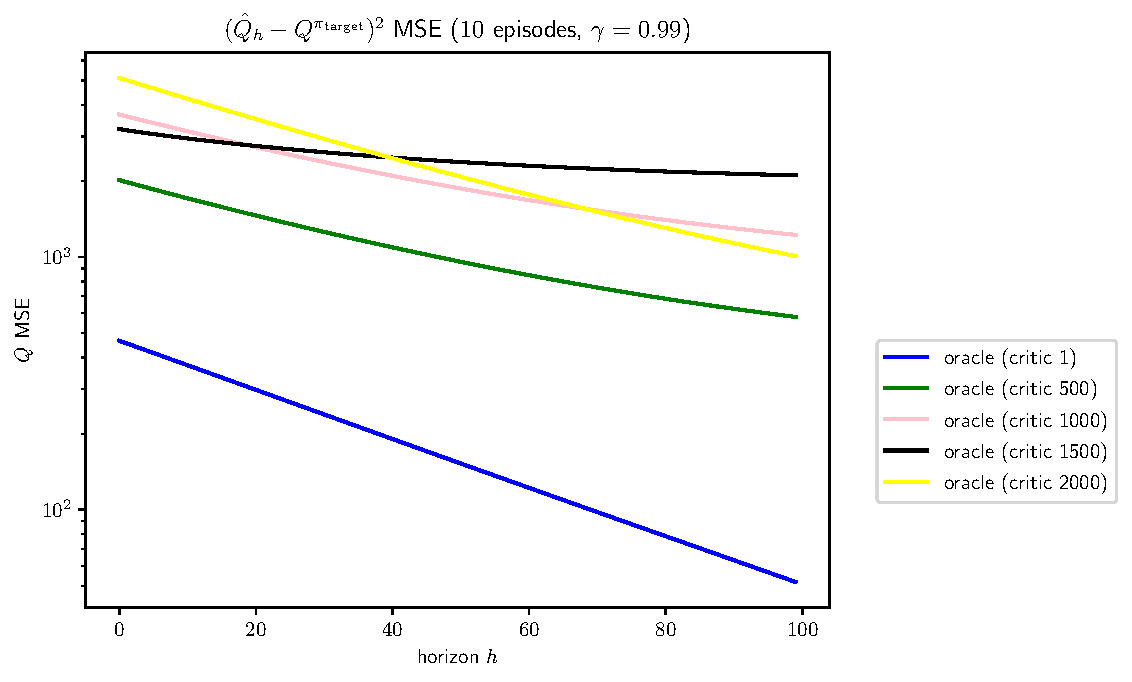
\includegraphics{cmp-mse.pdf}
\end{tikzfigure}

\textbf{Impact}. If successful, this can demonstrate utility of a new class of joint model-free and learned-model-based algorithms. Applications to robotic control are immediate.
}


\column{0.035}
\column{0.3}

\block[
  bodyoffsety=-1cm,
  titleoffsety=-1cm]{Model-Mixed DDPG}{
  Initialize $\pi, \hat\theta, \hat Q$. Loop:
  \begin{enumerate}
  \item Collect a sample playing $\pi$, add to replay buffer $B$.
  \item Update $\hat\theta$ with loss $\E \norm{s'-f_{\hat\theta}(s,a)}^2$, $(s,a,s')\sim B$
  \item Estimate $w(h)$ used in $\tilde Q$ (via sampling, holdout, or delta method)
  \item Update $\hat Q$ with loss $(\hat Q-\tilde Q)^2$ sampling from $B$.
  \item Update $\pi$ to maximize $\hat Q(s, \pi(s))$ for $s\in B$.
  \end{enumerate}
}
\block{Results Preview}{
  Fix ideal dynamics $\theta=\theta_\pi$ and $w(h)=\indicator\ca{h=5}$.

\begin{tikzfigure}[Comparison of MM-DDPG to DDPG on \texttt{HalfCheetah}.]
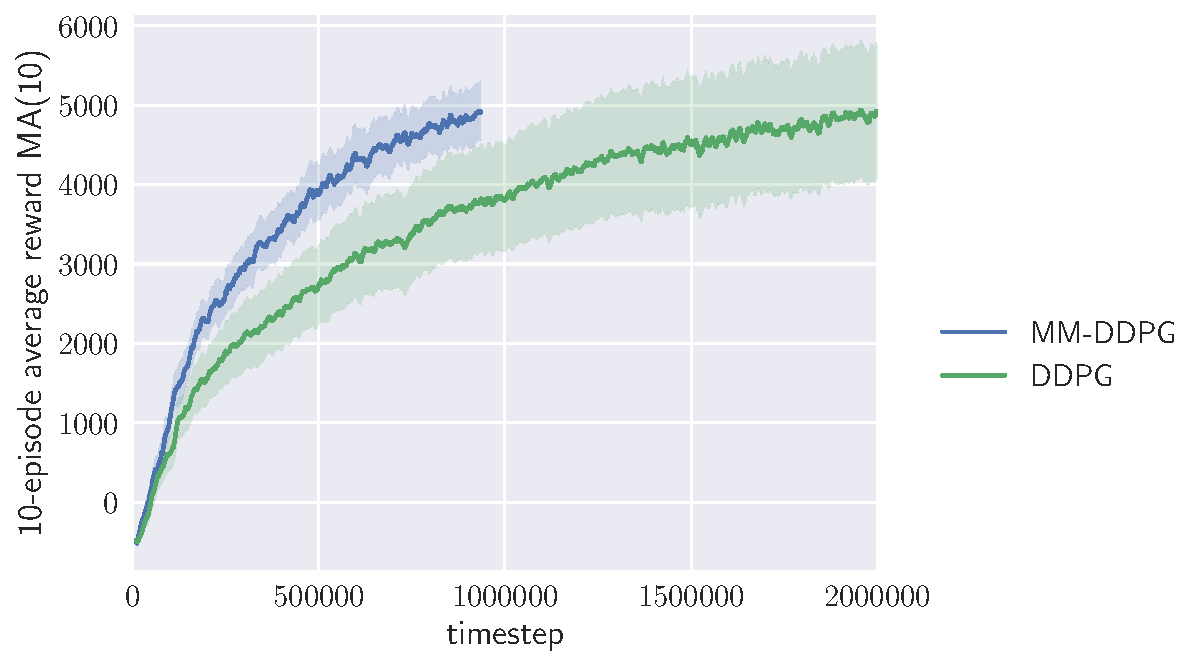
\includegraphics{ddpg-mh5.pdf}
\end{tikzfigure}
}
\block{Future Work}{
  \begin{itemize}
  \item Apply model-mixtures to other actor-critic algorithms, even policy-gradient ones.
  \item Theoretical results in probabilistic tabular setting with iterate-based analysis (Szepesv\'{a}ri 1997).
  \item Extend to constrained model-predictive control by learning $f$ which generalizes to actions near $\pi$, not just on $\pi$.
  \end{itemize}
}

\end{columns}
\end{document}
